\FloatBarrier
\section{The Compliance-Gated Dataset Class}

Administrative datasets generated by mandatory reporting programmes are not a homogeneous category. Some programmes create representative samples of the underlying population; others create samples that are structurally biased with respect to the outcome variable of interest. The distinction matters because the appropriate analytical treatment differs: a representative sample warrants standard regression or machine-learning workflows, whereas a structurally biased sample requires an explicit model of the selection process before any population-level claim can be made.

This section identifies the compliance-gated dataset, a specific subclass of mandatory reporting datasets whose structural properties are both analytically consequential and, crucially, analytically tractable.


\subsection{Formal Definition}

We work within the structural causal model (SCM) framework of \cit{pearletal2016}{Pearl et al. (2016, Section 1.5.1)} and \cit{pearl2009}{Pearl (2009, Definition 7.1.1)}. An SCM is a triple $\mathcal{M} = \langle U, V, \mathcal{F} \rangle$, where $U$ are exogenous background variables, $V$ are endogenous variables, and $\mathcal{F}$ is a set of structural equations assigning each endogenous variable to a function of its direct causes and a corresponding exogenous term.

For a compliance-gated dataset, let subscript $i$ index individual reporting units, let $X_i$ denote the full observed feature vector for unit $i$, and let $k$ denote the dimension of $\mathbf{X}_s$, equivalently the ambient dimension of the compliance region $\mathcal{R}$. The endogenous variables $V = \{\mathbf{X}_s, X_o, M, Y, C, M^{\text{obs}}, Y^{\text{obs}}\}$ are defined as follows, together with the compliance region $\mathcal{R}$, which parameterises the structural equation for $C$; among $V$, the first two form a partition of $X_i$, and the remaining five are outcome, compliance, and observation variables:

\par\medskip\noindent
{\small\itshape \textbf{Table 2.1. Variables of the compliance-gated SCM.} The endogenous variables of Definition 2.1, together with the compliance region $\mathcal{R}$ that parameterises the structural equation for $C$. The first two rows partition the observed feature vector $X_i$.\par}
\nopagebreak\medskip\nopagebreak
{
\setlength{\tabcolsep}{7pt}
\renewcommand{\arraystretch}{1.15}
\begin{longtable}{p{0.35\linewidth}lp{0.35\linewidth}}
\toprule
Symbol & Type & Role \\
\midrule
\endfirsthead
\toprule
Symbol & Type & Role \\
\midrule
\endhead
\bottomrule
\endlastfoot
$\mathbf{X}_{s,i} \subseteq X_i$ & vector & selection variables: determine compliance and cause $Y$ \\
$X_{o,i} = X_i \setminus \mathbf{X}_{s,i}$ & vector & non-selection features: always observed, may also cause $Y$ \\
$M_i$ & vector & latent mediators between $\mathbf{X}_s$ and $Y$ \\
$Y_i \in \mathbb{R}$ & scalar & outcome of interest: latent \\
$C_i \in \{0, 1\}$ & binary & compliance indicator: 1 if unit $i$ satisfies the reporting obligation \\
$M_i^{\text{obs}}$ & vector & analyst-observed mediators: $M_i$ if $C_i = 1$, missing otherwise \\
$Y_i^{\text{obs}} \in \mathbb{R}$ & scalar & analyst-observed outcome: $Y_i$ if $C_i = 1$, missing otherwise \\
$\mathcal{R} \subseteq \mathbb{R}^k$ & set & compliance region: $C_i = 1$ iff $\mathbf{X}_{s,i} \in \mathcal{R}$ \\
\end{longtable}
}
\par\medskip

Boldface is reserved for the selection vector $\mathbf{X}_s$, the quantity the gate reads; $X_o$ and $M$ are vectors as well, as Table 2.1 records, and are left unbold for legibility, while $Y$ and $C$ are scalars. The SCM equations that follow operate at the population level (no subscript $i$). The class definition treats $X_o$ as fully observed for all units; in practice, fields in $X_o$ with real missingness require a preprocessing step to reach full observability before this framework applies.

All structural equations in $\mathcal{F}$ take the causal assignment form $V \leftarrow f(\cdot)$: the left-hand side is the effect and the right-hand side contains its direct causes.

With this framework in place, we define the compliance-gated dataset class precisely.

\textbf{Definition 2.1 (Compliance-Gated Dataset).}

A compliance-gated dataset is the observational data $\mathcal{O} = \{\mathbf{X}_s, X_o, C, M^{\text{obs}}, Y^{\text{obs}}\}$, where each variable is generated by the following SCM, subject to the three conditions below.

\begin{align*}
    \mathbf{X}_s &\leftarrow U_{X_s} \\
    X_o &\leftarrow U_{X_o} \\
    M &\leftarrow f_M(\mathbf{X}_s,\; X_o,\; U_M) \\
    Y &\leftarrow f_Y(M,\; U_Y) \\
    C &\leftarrow \mathbf{1}\{ \mathbf{X}_s \in \mathcal{R} \} \\
    M^{\text{obs}} &\leftarrow C \cdot M \\
    Y^{\text{obs}} &\leftarrow C \cdot Y
\end{align*}

where $U_M$ and $U_Y$ are exogenous disturbances, mutually independent and independent of the upstream features; the upstream disturbances $U_{X_s}$ and $U_{X_o}$ are left unrestricted, so $\mathbf{X}_s$ and $X_o$ may be correlated. No result below uses their independence, since the analysis conditions on both, and Figure 2.1 draws them as separate roots only for legibility. The first four equations model the world; the last three model the institution: how the reporting obligation filters the world into a dataset. The conditions below serve two roles: Conditions 1 and 3 make explicit the institutional interpretation of equations already written above; Condition 2 imposes a genuine restriction on $f_M$, ruling out degenerate cases where $\mathbf{X}_s$ appears in $f_M$ with zero effect. An SCM with a different graph topology, or whose $f_M$ has zero effect for all $\mathbf{X}_s$ components, does not qualify as compliance-gated.

\begin{figure}[tbp]
\centering
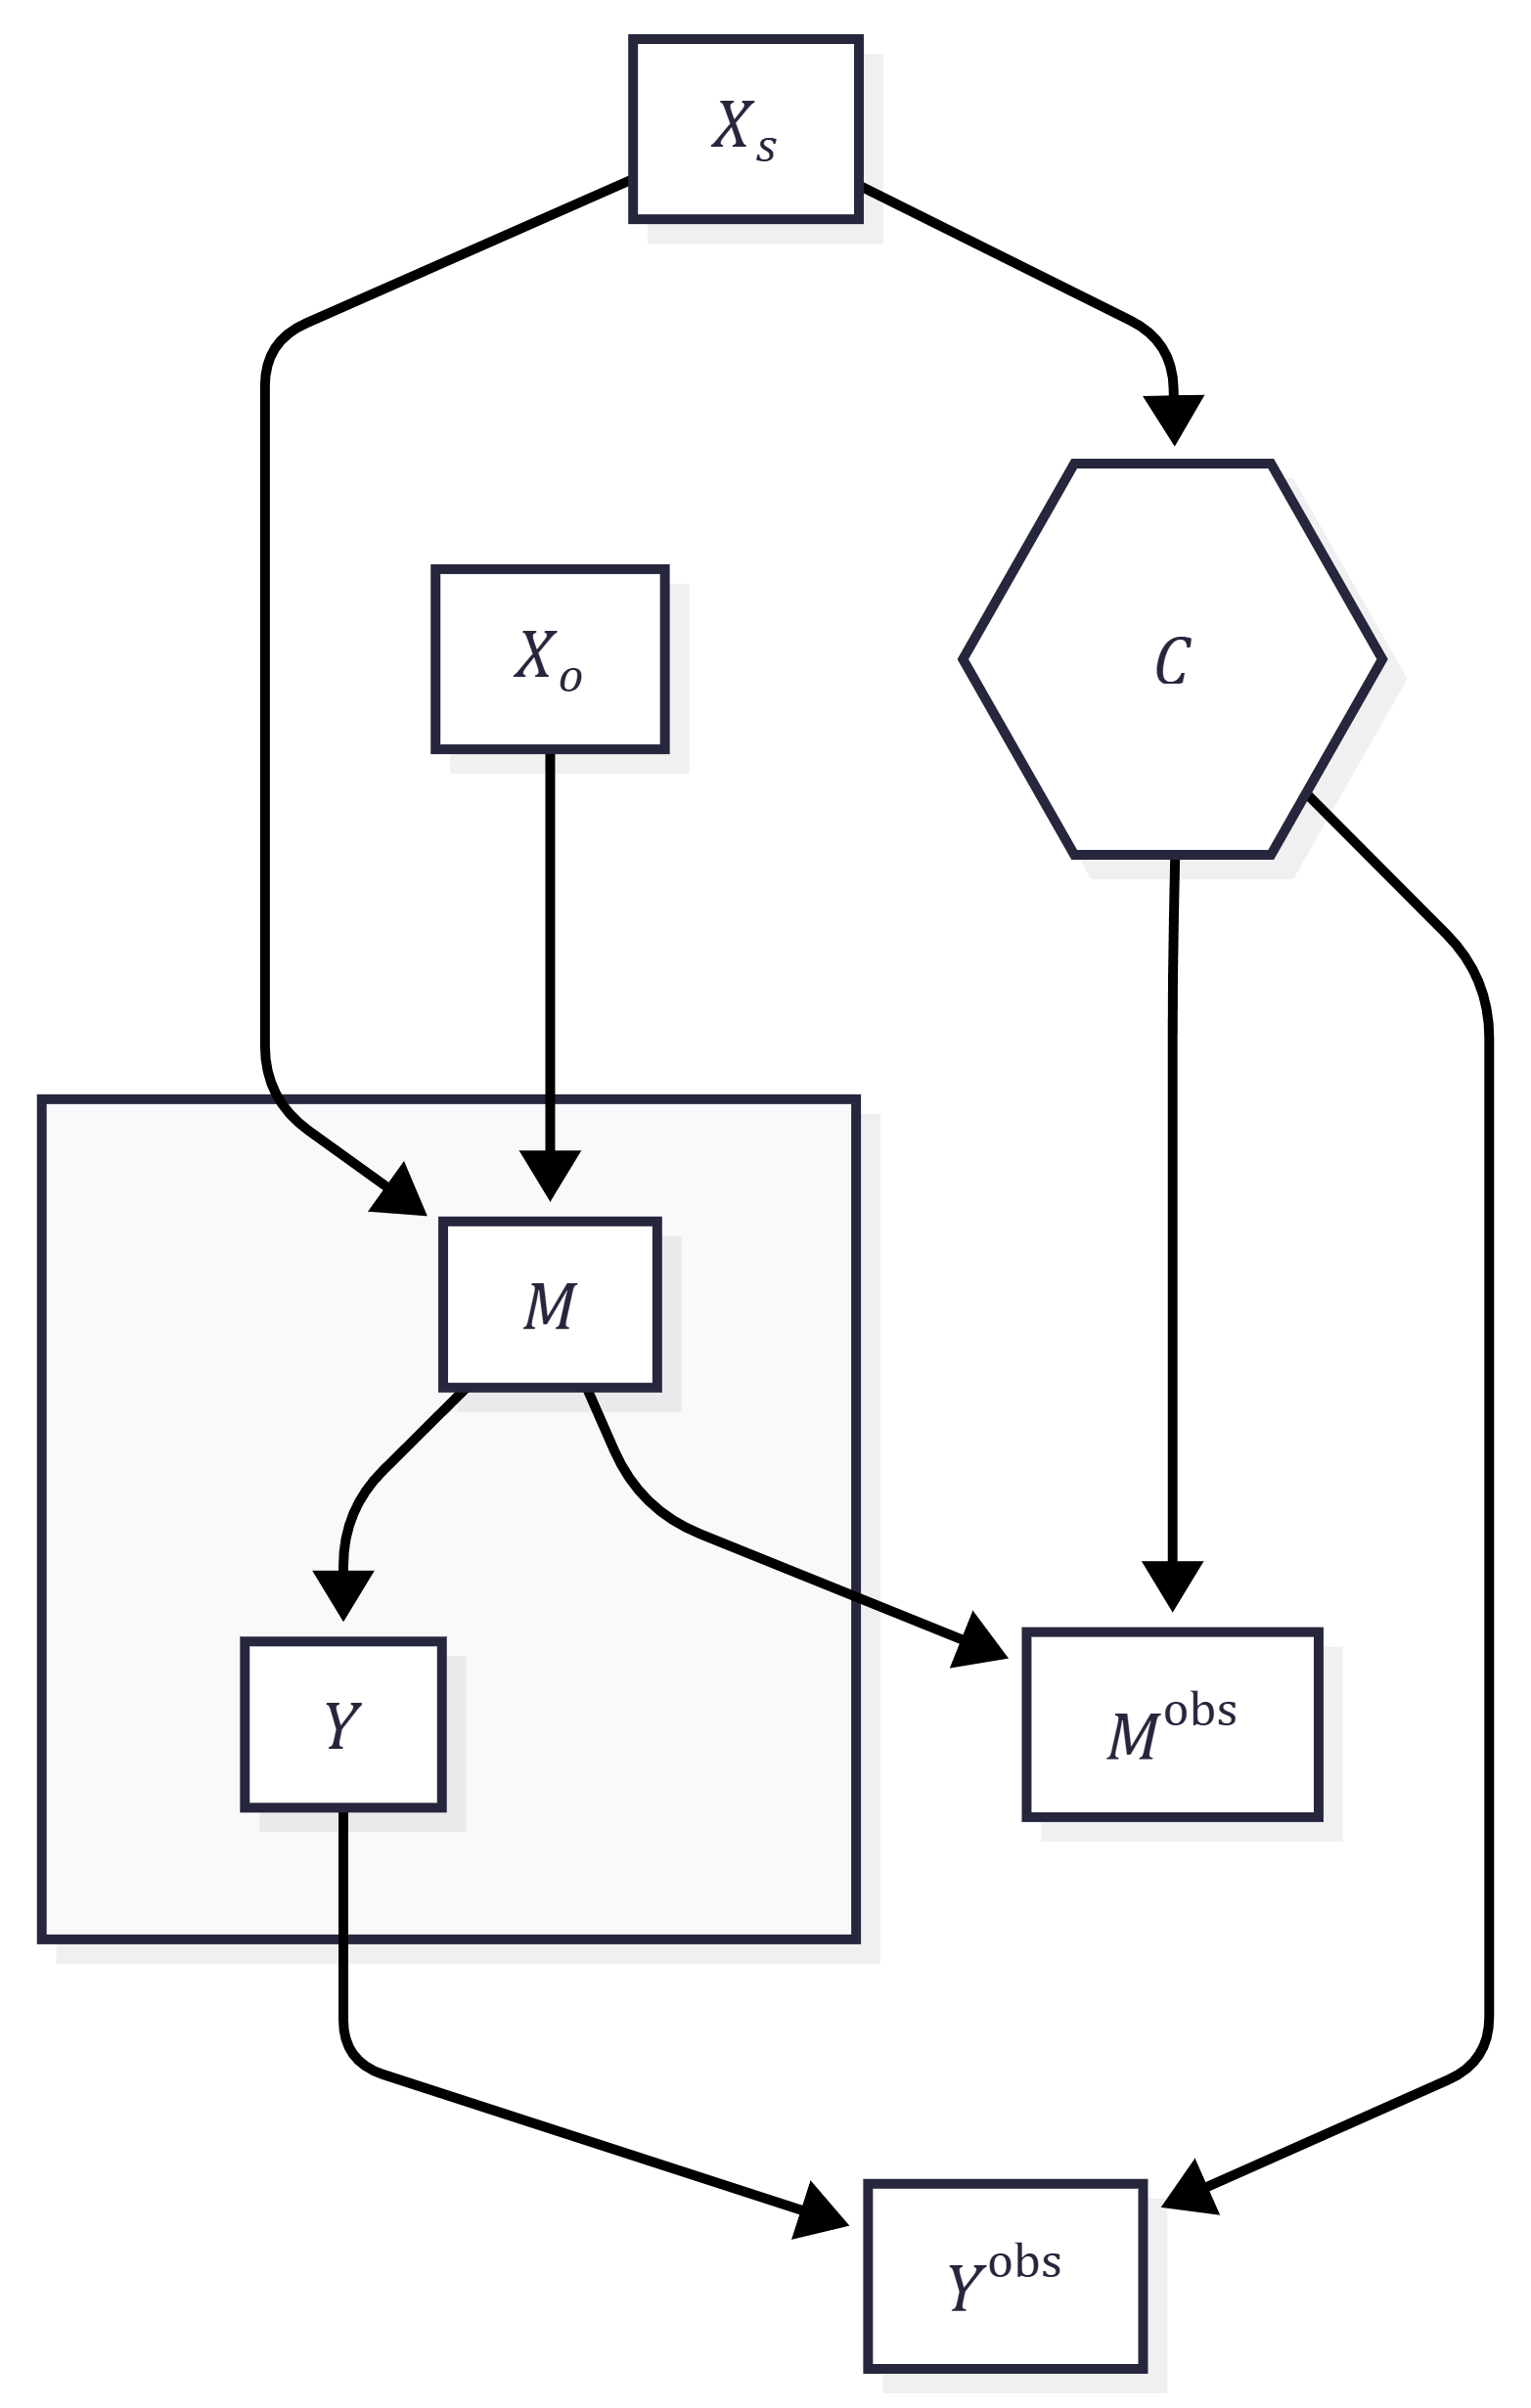
\includegraphics[width=0.425\linewidth]{figures/figure2_1.png}
\caption*{Figure 2.1. The causal DAG induced by the SCM in Definition 2.1 (exogenous $U$ nodes omitted). Four levels read top to bottom. Level 1: $\mathbf{X}_s$ and $X_o$, the upstream features, always observed for all units. Level 2: $C$, the compliance gate, with $\mathbf{X}_s$ as its sole parent; $X_o$ has no path to $C$. Level 3: $M$ and $Y$, the latent mediators and outcome; $M$ has parents $\mathbf{X}_s$ and $X_o$; $Y$ has $M$ as its sole parent; both exist for all units. Level 4: $M^{\text{obs}}$ and $Y^{\text{obs}}$, the analyst-observed quantities; each has two parents: the corresponding latent variable and $C$.}
\end{figure}

\textbf{Condition 1: Unit-level threshold selection.}

The compliance decision is made independently for each unit $i$ based solely on whether $\mathbf{X}_{s,i}$ falls within $\mathcal{R}$:

\[
C_i \leftarrow \mathbf{1}\{ \mathbf{X}_{s,i} \in \mathcal{R} \}.
\]

There is no discretion, no group-level assignment, and no partial compliance. Consequently, $Y_i^{\text{obs}}$ is non-missing if and only if $C_i = 1$.

Threshold-based programmes are the most common regulatory design. In such programmes, each selection variable $X_{s,j}$ is compared against a fixed threshold $T_j$, and the compliance region takes the form

\[
\mathcal{R} = \{ \mathbf{x} \in \mathbb{R}^k : x_j \geq T_j \text{ for all } j = 1, \ldots, k \},
\]

an intersection of half-spaces. Programmes that trigger compliance on any one criterion (OR logic) define $\mathcal{R}$ as a union of half-spaces instead. The formulation $\mathbf{X}_{s,i} \in \mathcal{R}$ accommodates both without modification.

This threshold-assignment rule is the same structure studied in regression discontinuity designs, where treatment switches as a running variable crosses a cutoff (\cit{leelemieux2010}{Lee \& Lemieux, 2010}). The two settings differ in aim: regression discontinuity uses the cutoff to identify a treatment effect among units near it, whereas Condition 1 uses it to determine which units are observed at all. Condition 1 also assumes that units do not manipulate $\mathbf{X}_s$ to select a side of the threshold. This assumption can fail when reporting is costly: the bunching literature documents units adjusting a choice variable to sit just below regulatory kinks and notches (\cit{kleven2016}{Kleven, 2016}). It is most secure when the selection variable is hard to manipulate, as with the gross floor area that gates the Chicago benchmarking obligation of Section 4.

\textbf{Condition 2: Endogenous selection variable.}

$\mathbf{X}_s$ appears as a causal argument in $f_M$ with non-zero effect: for at least one $j \in \{1, \ldots, k\}$, $f_M$ is non-constant in $X_{s,j}$, meaning there exist two values of $X_{s,j}$ that, with all other arguments of $f_M$ held fixed, yield different values of $M$. When $X_{s,j}$ is continuous and $f_M$ is differentiable, this is the familiar condition

\[
\frac{\partial f_M}{\partial X_{s,j}} \neq 0.
\]

The non-constancy form is the one the definition requires, since selection variables may be categorical, as with the property classes that co-determine the Chicago gate (Section 4), where a derivative is undefined.

Combined with $M \in \mathrm{pa}(Y)$ (the set of direct causal parents of $Y$ in the DAG) in the structural equation for $Y$, this guarantees at least one directed path $X_{s,j} \rightarrow M \rightarrow Y$ in the DAG induced by $\mathcal{F}$. The selection variables are not merely correlated with $Y$ through a common cause; they are causes of $Y$'s causal parents.

\textbf{Condition 3: Atomic reporting requirement.}

A unit reports all outcome data or none. For each unit $i$:

\[
M_i^{\text{obs}} = \begin{cases} M_i & \text{if } C_i = 1 \\ \emptyset & \text{if } C_i = 0 \end{cases}, \qquad Y_i^{\text{obs}} = \begin{cases} Y_i & \text{if } C_i = 1 \\ \emptyset & \text{if } C_i = 0 \end{cases}
\]

This restates what the SCM equations already encode: since $M^{\text{obs}}$ and $Y^{\text{obs}}$ are both gated by the same scalar $C$, partial reporting is structurally impossible.

The SCM implies that the analyst observes $\mathbf{X}_{s,i}$, $X_{o,i}$, and $C_i$ for every unit $i$, and additionally $M_i^{\text{obs}} = M_i$ and $Y_i^{\text{obs}} = Y_i$ for units with $C_i = 1$. Figure 2.1 above shows the causal DAG induced by Definition 2.1.

\textbf{Remark on necessity.}

Condition 1 alone produces a selected sample with MAR missingness, because $C$ is a deterministic function of observed $\mathbf{X}_s$. Yet it is not necessarily biased with respect to the $X$--$Y$ relationship. It is Condition 2 that makes the truncation analytically consequential: because $\mathbf{X}_s$ causes both selection and outcome, the compliant subsample is systematically enriched on $Y$ relative to the full population. Condition 3 distinguishes compliance-gated data from item non-response, where individual fields may be selectively missing. Their joint satisfaction produces the selection bias characterised in Section 2.2 and the documentation structure that makes DAG falsification tractable (Section 2.3).

Note that $f_M$ and $f_Y$ are left unspecified at the class level: the class definition constrains the causal graph structure and rules out degenerate $f_M$ (Condition 2), but leaves the specific functional forms of $f_M$ and $f_Y$ otherwise unspecified. Identifying the functional forms from institutional documentation is precisely the task of Stage 3 of the TDGP pipeline (Section 3.3). The scalar $Y$ likewise denotes a single factor of interest, the quantity a given study sets out to explain; a dataset may admit several such factors, each of the form $Y_k = f_{Y_k}(M)$, and the analyst instantiates the outcome role with whichever the research question selects (Section 3.2).

\textbf{Remark on the constitutive assumption.} The structural equations above are taken to be the rules the programme publishes, read from its governing documents (Section 2.3). The pipeline therefore rests on one premise: that the institution generates the data by the rules it sets down, so that those documents specify this structure with authority rather than merely describe it. The disturbance terms carry whatever the rules do not; a procedure applied with perfect uniformity would make $f_M$ and $f_Y$ deterministic, and the $U$ terms are the degree to which realized application departs from the documented rule. What the documents cannot supply is exogeneity: that these disturbances are mutually independent and uncorrelated with the features, the Markovian premise any structural model makes (\cit{pearl2009}{Pearl, 2009}), is assumed here as in any causal study, not read from a document. The constitutive premise occupies the place the asserted graph holds in an ordinary study, but on a firmer footing, an external authority rather than the analyst's judgement. Its further advantage is that it fails auditably: where the documented form leaves an empirical signal, a departure surfaces as a failed reconstruction or a gate discrepancy (Section 3.3) rather than in silence.

\subsection{The Selection Bias This Class Induces}

The analyst observes the set $\mathcal{O} = \{\mathbf{X}_s, X_o, C, M^{\text{obs}}, Y^{\text{obs}}\}$ and wants to study the outcome $Y$, to explain its variation and to predict it. The set is read unevenly: the upstream features and the compliance indicator are seen for every unit, but the outcome and the mediators only when $C = 1$, since $Y^{\text{obs}}$ and $M^{\text{obs}}$ are empty for all units with $C_i = 0$. The dataset is therefore not a sample drawn from a larger population; it may well cover the entire population, with the compliance gate acting as a missingness mechanism, not a sampling one.

Faced with this structure, an analyst has two paths. The first is to proceed with complete-case analysis: drop the units where $Y^{\text{obs}}$ is null and treat the remaining rows as sufficient for the analysis. This is the default behaviour of most statistical and machine-learning workflows, which silently discard incomplete rows. The second path is to treat the missingness as informative: to recognise that $Y^{\text{obs}} \neq Y$, that the units with absent outcomes are not random absences, and to actively correct for the difference. Proposition 2.1 below establishes formally how the first path fails. 

\textbf{Proposition 2.1 (Compliance-Gate Selection Bias).} Under Definition 2.1, suppose

(i) $P(\mathbf{X}_s \in \mathcal{R}) \in (0,1)$: the population contains both compliant and non-compliant units; and

(ii) $E[Y \mid C = 1] \neq E[Y \mid C = 0]$: the two compliance groups differ in expected outcome.

Then the expected outcome among compliant units differs from the population expected outcome:

\[
E[Y \mid C = 1] \neq E[Y].
\]

\textit{Proof.} The compliance criterion partitions the population into compliant units ($\mathbf{X}_s \in \mathcal{R}$) and non-compliant units ($\mathbf{X}_s \notin \mathcal{R}$). By the law of total expectation,

\[
E[Y] = E[Y \mid C = 1]\, P(C = 1) + E[Y \mid C = 0]\, P(C = 0).
\]

Suppose for contradiction that $E[Y \mid C = 1] = E[Y]$. Substituting and rearranging gives $E[Y \mid C = 1]\, P(C = 0) = E[Y \mid C = 0]\, P(C = 0)$, and since $P(C = 0) > 0$ by (i), this forces $E[Y \mid C = 1] = E[Y \mid C = 0]$, contradicting (ii). The compliance gate sets $Y^{\text{obs}} = \emptyset$ for all units with $\mathbf{X}_s \notin \mathcal{R}$, so complete-case analysis retains only the compliant group and computes $E[Y \mid C = 1]$, which is not $E[Y]$. $\square$

\textbf{Remark on condition (ii).} Condition (ii) is where Condition 2 of Definition 2.1 does its work, and the proposition states it as a hypothesis rather than deriving it, because the derivation does not go through as pure logic. Condition 2 guarantees that $f_M$ is non-constant in at least one component of $\mathbf{X}_s$, so the two groups pass systematically different inputs through the same structural functions: compliant units draw $\mathbf{X}_s$ from within $\mathcal{R}$, non-compliant units from outside it. What Condition 2 does not rule out is exact cancellation, since a non-constant function can still average to the same value over two disjoint regions. Equality of the two group means would require the variation of $f_M$ across the threshold to cancel exactly against the distribution of $\mathbf{X}_s$, a knife-edge that nothing in the institutional design protects and that any perturbation of the input distribution would break. Condition (ii) is therefore the generic case for the class. For the threshold programmes that motivate it, the case is stronger still: a programme gates on a measure of scale precisely because scale drives the outcome it exists to measure, so units above the threshold are enriched on $Y$ by the programme's own design logic. Section 4 exhibits the difference directly in the Chicago data, where compliant buildings are systematically larger and emissions scale near-proportionally with size.

The error arises at the inferential step. $Y^{\text{obs}}$ is not wrong: for every compliant unit, $Y_i^{\text{obs}} = Y_i$ exactly, and the complete cases are internally consistent. The error is not in the data but in what the analyst does with it: using statistics computed from $Y^{\text{obs}}$ as if they described the full population, when in fact they describe only the subset of units whose outcomes were made observable by the compliance gate.

From the analyst's perspective, the error is invisible at the analysis stage. The complete cases look like a coherent dataset: the rows are fully populated, the model converges, the metrics are reasonable. Nothing in the output signals that non-compliant units exist or that their outcomes were systematically different from those of compliant units. The bias is structural, a property of the institutional rule that generated the data rather than of the analysis itself, and it persists regardless of sample size. Even if the analyst had records for every unit in the population, the compliance gate would still withhold $Y$ for every non-compliant unit, leaving the bias exactly as severe. A better or larger sample is not the answer; the missing values are not absent by chance, and no amount of data can supply what the compliance gate withholds.

The cause of missingness determines the correction. Knowing that the bias exists is not sufficient to correct it. The form of the correction depends on what drives the missingness, specifically on whether the probability of a unit's outcome being absent depends on the outcome itself or only on other observed variables. Different answers lead to different corrections, and some missingness patterns are not correctable at all from observed data alone.

To classify the mechanism, introduce $R_i = 1 - C_i$ as the missingness indicator for unit $i$: $R_i = 1$ when $Y_i^{\text{obs}}$ is absent, $R_i = 0$ when observed. \cit{rubin1976}{Rubin (1976)} distinguishes three categories based on what $P(R_i = 1 \mid Y_i, \mathbf{X}_{s,i}, X_{o,i})$ depends on. Under \textbf{MCAR} (Missing Completely At Random), the probability of missingness is unrelated to any characteristic of the unit; absences are literally random. Under \textbf{MAR} (Missing At Random), missingness depends only on observed variables: once those are conditioned on, the absent value carries no additional information about why it is missing. Under \textbf{MNAR} (Missing Not At Random), the probability of missingness depends on the unobserved value $Y_i$ itself: for example, firms with worse financial outcomes selectively withhold voluntary disclosure, making the absent values informative in a way that cannot be recovered from observed data alone.

Compliance-gate data is MAR. From the SCM, the compliance decision is made by comparing $\mathbf{X}_{s,i}$ against $\mathcal{R}$. Nothing about $Y_i$ enters that decision. The probability that unit $i$'s outcome is absent is:

\[
P(R_i = 1 \mid Y_i,\, \mathbf{X}_{s,i},\, X_{o,i}) = \mathbf{1}\{\mathbf{X}_{s,i} \notin \mathcal{R}\}.
\]

In this expression, the left-hand side is the probability of missingness given full knowledge of the unit, including its latent $Y_i$. The right-hand side is the indicator that $\mathbf{X}_{s,i}$ falls outside $\mathcal{R}$, a function only of the always-observed $\mathbf{X}_{s,i}$. The value of $Y_i$ on the left plays no role. Once $\mathbf{X}_{s,i}$ is known, the compliance decision is deterministic: the conditional probability is 0 or 1, not a number between them. This is MAR: the missingness is fully explained by an observed variable, and the missing outcome values carry no additional information about why they are absent.

The MAR classification is consequential. Because the missingness mechanism is fully characterised by $\mathbf{X}_s$, it can be modelled using the data already in hand. Estimating the probability that a unit was required to report, $P(C = 1 \mid \mathbf{X}_s, X_o)$, and reweighting the complete cases by its inverse corrects the bias across the region the gate leaves populated. Treated this way, the missingness indicator $R$ is itself a node in the causal graph, placing the analysis within the missingness-graph framework of \cit{mohanpearl2021}{Mohan and Pearl (2021)}, whose graphical criteria identify when a target distribution is recoverable from incomplete data. The reweighting reaches only as far as that overlap: where the threshold leaves no compliant units to carry the weight, the target is not recoverable by reweighting alone, and recovery there passes to the structural form (Section 3.4). A further assumption underwrites the correction even within the overlap: the deterministic gate makes selection ignorable given $\mathbf{X}_s$ by construction, but where realized compliance departs from the documented rule, that ignorability becomes an assumption on the observed features rather than a consequence of the gate (Sections 3.1, 3.4). This is the logic of inverse probability weighting, which Section 5 implements.

The MAR structure also locates this class relative to the econometric sample-selection tradition. \cit{heckman1979}{Heckman (1979)} treats selection bias as a specification error and corrects it with a two-step estimator; that machinery is built for samples whose selection may depend on unobservables correlated with the outcome equation, the MNAR configuration, and in its classical form it buys identification with distributional assumptions on the joint error structure or an exclusion restriction. The compliance gate needs none of that apparatus: selection is a documented, deterministic function of observed covariates, so the missingness is MAR and inverse probability weighting on an estimated propensity identifies the recoverable region without distributional assumptions on the outcome equation. That economy is a direct payoff of the class structure rather than a methodological preference. The two approaches remain complements: where realized compliance departs from the documented rule in ways that track unobservables, the configuration drifts toward the one Heckman's estimator was built for, and the selection-ignorability assumption of Section 3.4 is what bounds that drift.

Cross-validation does not detect this bias. In a standard $k$-fold cross-validation, both training and test folds are drawn from the complete cases, the units where $Y^{\text{obs}}$ is non-null. The test fold is subject to the same compliance gate as the training fold: it contains only units with $\mathbf{X}_s \in \mathcal{R}$, not a draw from the full population. What cross-validation measures is how well the model captures $E[Y \mid \mathbf{X}_s, X_o, C = 1]$, the conditional expectation within the compliant subsample. A model can achieve excellent performance on this criterion while still producing biased estimates of the population-level $E[Y \mid \mathbf{X}_s, X_o]$. Cross-validation tests model fit on the complete cases; it does not test whether the complete cases are representative of the population.

\subsection{Why DAG Falsification Is Tractable for This Class}

The central obstacle to applied causal inference is not estimation but specification. Once a directed acyclic graph (DAG) is fixed, Pearl's framework converts identification questions into estimation procedures: the do-calculus rewrites interventional quantities such as $P(Y \mid do(X))$ in terms of observational quantities whenever the DAG permits; the back-door and front-door criteria pick out which variables to adjust for in order to block confounding paths or to exploit a fully observed mediating chain; counterfactual identification extends the same machinery to queries about what would have happened under alternative interventions. Every step in this pipeline rests on a single explicit assumption: that the DAG faithfully represents the data-generating process. Once that assumption is granted, the rest follows mechanically. The difficulty lies upstream, at the point where the DAG itself is proposed. In most observational studies, the DAG is asserted on the basis of subject-matter expertise: the analyst draws arrows between variables, defends the choices in prose, and proceeds. The arrows are not derived from an authoritative external source, and observational data alone is generally insufficient to distinguish between DAGs that imply incompatible causal estimands (\cit{pearl2009}{Pearl, 2009, Ch. 2}). This is the DAG falsification problem.

Compliance-gated datasets are unusual in this regard. The documentation is constitutive, not descriptive: legislation, regulatory rules, and technical reporting standards are the \textit{primary source} of the compliance obligation, not a secondary description of it. A building falls under a benchmarking ordinance because the ordinance text says it does; a firm files a financial disclosure because the SEC rules say it must. The institutional documents are in force before any data is collected, and they specify in operational detail what must be reported, by whom, and how the reported quantities are calculated. This documentation is not commentary on the data-generating process; it is the written specification of the institutional rules that produce the dataset.

Three components of the DAG induced by Definition 2.1 map directly onto three components of this documentation. The selection rule, which determines which units must report and on what criterion, is specified by the threshold provision of the regulation; this is exactly Condition 1 of Definition 2.1, and it identifies $\mathbf{X}_s$, $\mathcal{R}$, and the structural equation for $C$. The reporting schema, which determines which variables must be filed by compliant units, is specified by the regulation's enumeration of required fields; this identifies $M^{\text{obs}}$ and $Y^{\text{obs}}$, and through them the latent $M$ and $Y$. The functional structure linking reported variables to the outcome, typically given as an accounting formula, emissions factor, or measurement standard, is specified by the technical annex of the regulation; this identifies $f_Y$ and the parent set $\mathrm{pa}(Y)$. These three mappings cover exactly what Definition 2.1 leaves to be supplied per application: the identities of $\mathbf{X}_s$, $M$, and $Y$; the compliance region $\mathcal{R}$; and the functional form $f_Y$. The class definition and the documentation are complementary by construction: the SCM provides the skeleton, the documentation provides the flesh.

One structural feature lies outside this correspondence: the upstream-to-mediator edges $\mathbf{X}_s \to M$ and $X_o \to M$, by which the upstream features produce the mediators. The mediators are measured, not computed from a rule, so no document constitutes these links; they are confirmed the ordinary way, by checking that the upstream features predict $M$ in the data. That they rest on association rather than the constitutive source is harmless, because they bear on whether the bias exists, not on whether the correction is valid. For the bias to exist the analysis needs only that $\mathbf{X}_s$ be among the causes of $M$ (Condition 2), which the data settle directly; the validity of the correction rests instead on the documented gate, on $\mathrm{pa}(Y) = M$, and on selection being ignorable given the observed features (Section 3.4), and the analysis conditions on $X_o$ whether or not $X_o \to M$ holds.

The consequence is that the DAG becomes testable, not merely assertable. Because the documentation supplies the very components the graph hypothesises, each conjecture can be set against the provision that fixes it: a conjectured selection variable against the threshold provision, a conjectured mediator or outcome against the reporting schema, the parent set of $Y$ against the technical formula. A conjecture the documentation contradicts is refuted, and the provision that contradicts it names the correction, so the candidate graph can be brought into line with the source rather than merely defended. This is a test against an authoritative external standard, and it reaches a conclusion that argument from domain expertise alone cannot. One of the three components leaves an empirical mark as well: because the formula computes $Y$ from $M$, the documented mediators should reconstruct the reported outcome within the compliant subset, so the data can corroborate $\mathrm{pa}(Y) = M$ on that one link. These three components, though, are settled by the documents whether or not that mark is read.

In a general observational dataset, no equivalent primary source exists. The substitutes available to the analyst are codebooks, expert opinion, and prior literature, and each falls short. A codebook documents fields, not causal relationships. Subject-matter experts can be consulted, but expert opinion is contestable and does not produce a falsifiable functional form. Prior literature can be invoked, but it inherits the same problem one step removed: the DAGs proposed in earlier studies were themselves typically asserted by their authors rather than tested against an external source, and grounding a new DAG on them only chains one assertion to another without anchoring the structure in anything that could refute the chain.

This tractability is what justifies treating compliance-gated datasets as a distinct analytical class. The DAG must still be subjected to a falsification test, since that work does not happen automatically, but the ingredients required to carry it out are present in the documentation. Section 3 operationalises this insight; Section 4 carries it out on the Chicago Energy Benchmarking dataset.

\subsection{Scope of the Class}

This section shows that real reporting programmes belong to the class. Mandatory-reporting regimes across energy, labour, environmental, and financial regulation all satisfy the three conditions of Definition 2.1. The Chicago benchmarking data of Section 4 is therefore one instance of the class rather than the whole of it.

The common pattern is a size threshold. Regulators rarely impose reporting obligations uniformly. They exempt small units to limit administrative burden and target the units whose activity dominates the outcome the programme exists to measure. The exemption is written as a threshold on an observable measure of scale, and that same measure of scale is a cause of the outcome. This is precisely the configuration of Conditions 1 and 2: the selection variable is a threshold-gated measure of size (Condition 1), and size drives the reported outcome through the programme's mediators (Condition 2). Table 2.2 maps four programmes onto the class.

\par\medskip\noindent
{\small\itshape \textbf{Table 2.2. Four compliance-gated reporting programmes mapped onto Definition 2.1.} Each programme gates a reported outcome on a size threshold, and the selection variable is a cause of that outcome. The final column names the constitutive document that, per Section 2.3, encodes the selection rule, the reporting schema, and the outcome's functional form.\par}
\nopagebreak\medskip\nopagebreak
{
\footnotesize
\setlength{\tabcolsep}{5pt}
\renewcommand{\arraystretch}{1.15}
\begin{longtable}{>{\raggedright\arraybackslash}p{\dimexpr 0.146\linewidth-2\tabcolsep\relax}>{\raggedright\arraybackslash}p{\dimexpr 0.146\linewidth-2\tabcolsep\relax}>{\raggedright\arraybackslash}p{\dimexpr 0.356\linewidth-2\tabcolsep\relax}>{\raggedright\arraybackslash}p{\dimexpr 0.2\linewidth-2\tabcolsep\relax}>{\raggedright\arraybackslash}p{\dimexpr 0.152\linewidth-2\tabcolsep\relax}}
\toprule
Programme & Selection variable $\mathbf{X}_s$ & Compliance region $\mathcal{R}$ & Reported outcome $Y$ (via mediators $M$) & Constitutive document \\
\midrule
\endfirsthead
\toprule
Programme & Selection variable $\mathbf{X}_s$ & Compliance region $\mathcal{R}$ & Reported outcome $Y$ (via mediators $M$) & Constitutive document \\
\midrule
\endhead
\bottomrule
\endlastfoot
Municipal energy benchmarking & Gross floor area & Area $\geq$ threshold (50,000 sq ft in Chicago) & GHG emissions, via metered fuel use & Benchmarking ordinance; EPA emission-factor tables \\
OSHA injury recordkeeping & Establishment employee count & More than 10 employees, outside exempt industries & Recordable injury and illness counts, via worker-hours of exposure & 29 CFR Part 1904 \\
EPA Toxics Release Inventory & Employee count \textit{and} chemical throughput & $\geq$ 10 FTE-equivalents AND > 25,000 lb manufactured/processed (or > 10,000 lb otherwise used) of a listed chemical & Annual chemical releases, via production volume & EPCRA §313; 40 CFR Part 372 \\
SEC accelerated-filer disclosure (boundary case) & Public float & Public float $\geq$ \$75 million & Enhanced financial disclosures, via firm scale of operations & Exchange Act Rule 12b-2 (17 CFR §240.12b-2) \\
\end{longtable}
}
\par\medskip

\textit{Boundary case:} SEC disclosure satisfies Conditions 1 and 2, but Condition 3 only for individual gated items, not the filing as a whole (see below).

Municipal energy benchmarking, the first row of the table, is the member that Section 4 develops in full using the Chicago Energy Benchmarking data. This section works through the other three. Taken in turn, OSHA recordkeeping, the EPA Toxics Release Inventory, and SEC disclosure show both the range of the class and where its conditions bind.

\textbf{OSHA injury recordkeeping.} An establishment with ten or fewer employees at all times in the prior calendar year is partially exempt from injury and illness recordkeeping (\cit{osha2001}{OSHA, 2001, §1904.1}), as are establishments in designated low-hazard industries (§1904.2). Employee count is the selection variable, and the threshold defines $\mathcal{R}$ (Condition 1). It also causes the outcome: more employees mean more worker-hours of exposure, and recordable injuries accumulate with exposure, so selection acts on the outcome through an operational-scale mediator (Condition 2). A unit keeps the full log or none, the atomic requirement of Condition 3. Complete-case analysis over the recorded establishments would describe injury rates among larger firms, not the full population of workplaces.

\textbf{EPA Toxics Release Inventory.} The TRI is the cleanest illustration of the AND-logic compliance region of Condition 1. A facility must file an annual release report only if it meets three criteria at once (U.S. EPA, 40 CFR §372.22): it operates in a covered industry sector, employs the equivalent of ten or more full-time staff, and manufactures or processes more than 25,000 pounds, or otherwise uses more than 10,000 pounds, of a listed chemical (40 CFR §372.25). The region $\mathcal{R}$ is thus an intersection of half-spaces. Chemical throughput, one component of $\mathbf{X}_s$, directly causes releases: a facility that processes more of a chemical has more to release. Condition 2 holds through this path, and releases are gated atomically with the rest of the Form R, satisfying Condition 3.

\textbf{SEC disclosure thresholds.} SEC disclosure partially qualifies, and marks the boundary of the class. Conditions 1 and 2 hold: Exchange Act Rule 12b-2 (SEC, 17 CFR §240.12b-2) classifies an issuer as an accelerated filer once its public float reaches \$75 million, and public float scales with the operations that generate the disclosed financials. Condition 3 does not hold for the filing as a whole, because every public issuer files a Form 10-K regardless of size; the threshold toggles the stringency of disclosure, not its existence. Membership holds only at the level of an individual gated item, such as the auditor's attestation on internal control over financial reporting, which appears above the threshold and is absent below it.

All four examples supply what the falsification test of Section 2.3 needs: a constitutive document in force before any data was collected. The benchmarking ordinance points to the EPA emission-factor tables; the TRI rules incorporate published release-estimation methods; OSHA's regulation defines what counts as a recordable case. Wherever such a document exists, the DAG can be tested rather than merely asserted.

These programmes are illustrative, not a complete inventory. The criterion they share is general: a written rule that predates the data, fixes which units are recorded, and turns on a cause of the outcome. Nothing about that criterion is peculiar to government regulation. Many private-sector datasets are generated the same way. Consider a lender's loan book. The selection variable $\mathbf{X}_s$ is the applicant's credit score; the compliance region $\mathcal{R}$ is the set of scores at or above the approval cutoff written into the lender's credit policy; and the reported outcome $Y$ is repayment behaviour, recorded only for the applicants the cutoff admits. The credit policy is fixed before any loan is issued, and the score that triggers approval is itself a cause of repayment, so Conditions 1 and 2 hold exactly as in the regulatory cases. The same structure recurs wherever a written rule decides what is recorded: an insurer underwriting from an eligibility manual, a clinical registry enrolling only patients who meet pre-specified inclusion criteria, a marketplace logging only the transactions its published rules permit. Each is governed by a process fixed before the data exists, and each gates observation on a variable that also drives the outcome.

What defines membership, then, is not the domain, nor whether the governing rule is public law or internal policy, but whether the analyst can obtain the document that states it. When that document is available, as it is for the regulatory programmes above, the data-generating process is recoverable and the falsification test of Section 2.3 can be run. When it is proprietary and withheld, the process is still constitutive but no longer recoverable, and the dataset falls back to the ordinary observational case in which the DAG can only be asserted. The class is broad on this criterion, and the pipeline of Section 3 applies to any member whose governing document can be read; the Chicago Energy Benchmarking data is simply where this paper carries the procedure out in full.

